\section{构建阀盖三维模型}
\begin{procedure}
\item 切换视图方向为西南等轴测图。
\item 拉伸构建$\phi 5$圆柱,其结果如图\ref{fig:fagai9}所示。
\begin{figure}[htbp]
\centering
\subfloat[]{\label{fig:fagai9}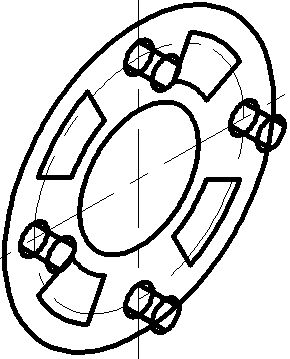
\includegraphics[scale=0.4]{fagai9.png}}\hspace{30pt}
\subfloat[]{\label{fig:fagai10}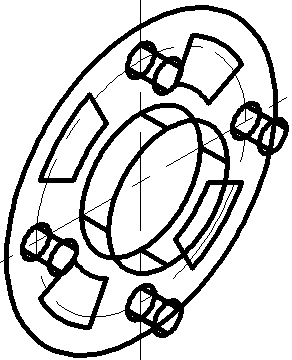
\includegraphics[scale=0.4]{fagai10.png}}\\
\subfloat[]{\label{fig:fagai11}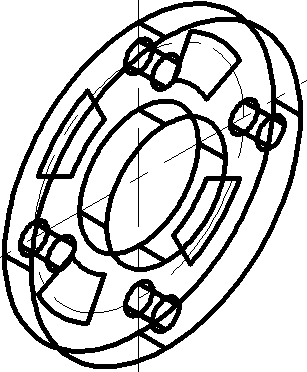
\includegraphics[scale=0.4]{fagai11.png}}\hspace{30pt}
\subfloat[]{\label{fig:fagai12}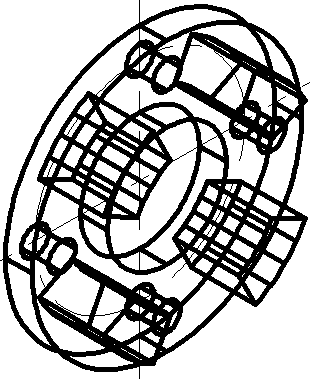
\includegraphics[scale=0.4]{fagai12.png}}\\
\caption{阀盖拉伸过程}
\end{figure}
\begin{lstlisting}
|命令: EXTRUDE|
|当前线框密度:  ISOLINES=4,闭合轮廓创建模式 = 实体|
|选择要拉伸的对象或 [模式(MO)]: 找到 1 个|
|选择要拉伸的对象或 [模式(MO)]: 找到 1 个,总计 2 个|
|选择要拉伸的对象或 [模式(MO)]: 找到 1 个,总计 3 个|
|选择要拉伸的对象或 [模式(MO)]: 找到 1 个,总计 4 个|
|选择要拉伸的对象或 [模式(MO)]:|
|指定拉伸的高度或 [方向(D)/路径(P)/倾斜角(T)/表达式(E)]: 5|
\end{lstlisting}

\item 拉伸构建$\phi 22$圆柱,其结果如图\ref{fig:fagai10}所示。
\begin{lstlisting}
|命令:EXTRUDE|
|当前线框密度:  ISOLINES=4,闭合轮廓创建模式 = 实体|
|选择要拉伸的对象或 [模式(MO)]: 找到 1 个|
|选择要拉伸的对象或 [模式(MO)]:|
|指定拉伸的高度或 [方向(D)/路径(P)/倾斜角(T)/表达|
|式(E)] $<$5.0000$>$:|
\end{lstlisting}
\item 拉伸构建$\phi 50$圆柱,其结果如图\ref{fig:fagai11}所示。
\begin{lstlisting}
|命令:EXTRUDE|
|当前线框密度:  ISOLINES=4,闭合轮廓创建模式 = 实体|
|选择要拉伸的对象或 [模式(MO)]: 找到 1 个|
|选择要拉伸的对象或 [模式(MO)]:|
|指定拉伸的高度或 [方向(D)/路径(P)/倾斜角(T)/表达|
|式(E)] $<$5.0000$>$:|
\end{lstlisting}
\item 拉伸构建阀盖定位块,其结果如图\ref{fig:fagai12}所示。
\begin{lstlisting}
|命令: EXTRUDE|
|当前线框密度:  ISOLINES=4,闭合轮廓创建模式 = 实体|
|选择要拉伸的对象或 [模式(MO)]: 找到 1 个|
|选择要拉伸的对象或 [模式(MO)]: 找到 1 个,总计 2 个|
|选择要拉伸的对象或 [模式(MO)]: 找到 1 个,总计 3 个|
|选择要拉伸的对象或 [模式(MO)]: 找到 1 个,总计 4 个|
|选择要拉伸的对象或 [模式(MO)]:|
|指定拉伸的高度或 [方向(D)/路径(P)/倾斜角(T)/表达|
|式(E)]$<$5.0000$>$: 12|
\end{lstlisting}
\item 进行差集操作。

从$\phi 50$圆中减去四个$\phi 5$的圆和一个$\phi 22$的圆。
\begin{lstlisting}
|命令: subtract |
|选择要从中减去的实体、曲面和面域...|
|选择对象: 找到 1 个|
|选择对象:  选择要减去的实体、曲面和面域...|
|选择对象: 找到 1 个|
|选择对象: 找到 1 个,总计 2 个|
|选择对象: 找到 1 个,总计 3 个|
|选择对象: 找到 1 个,总计 4 个|
|选择对象: 找到 1 个,总计 5 个|
|选择对象:|
\end{lstlisting}
\item 进行合并实体操作。

合并实体需要用到AutoCAD中的并集命令,启动实体【并集】命令的方法有:
\begin{itemize}
\item 键盘输入UNION\index{union}或UNI。
\item 【修改】$\rightarrow$【实体编辑】$\rightarrow$【并集】。
\item 【实体编辑】$\triangleright$【并集】图标
\includegraphics[scale=0.7]{union.png}。
\end{itemize}
\begin{lstlisting}
|命令: UNION|
|选择对象: 指定对角点: 找到 5 个|
|选择对象:|
\end{lstlisting}
\item 设置视觉样式为灰度,其结果如图\ref{fig:fagailititu}所示。
\item 将端盖模型保存为“调压阀阀盖立体图.dwg”。
\end{procedure}
\begin{figure}[htbp]
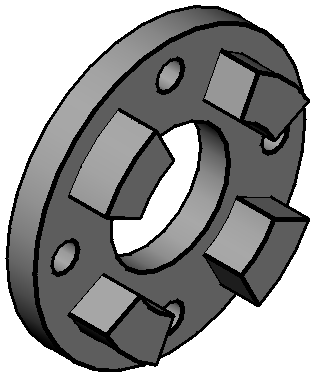
\includegraphics[scale=0.6]{fagailititu.png}
\caption{阀盖三维模型}\label{fig:fagailititu}
\end{figure}
\endinput